\documentclass{article}
\usepackage{tikz}
\usetikzlibrary{arrows}

\tikzset{
  treenode/.style = {align=center, inner sep=0pt, text centered,
    font=\sffamily},
  arn_n/.style = {treenode, circle, white, font=\sffamily\bfseries, draw=black,
    fill=black, text width=1.5em},% arbre rouge noir, noeud noir
  arn_r/.style = {treenode, circle, red, draw=red, 
    text width=1.5em, very thick},% arbre rouge noir, noeud rouge
  arn_x/.style = {treenode, rectangle, draw=black,
    minimum width=0.5em, minimum height=0.5em}% arbre rouge noir, nil
}

\begin{document}
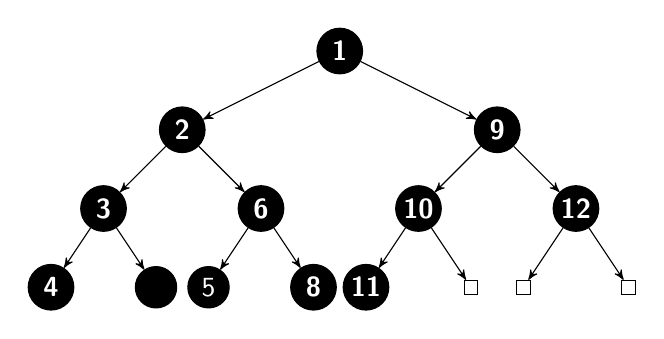
\begin{tikzpicture}[->,>=stealth',level/.style={sibling distance = 4cm/#1,
  level distance = 1.cm}] 
\node [arn_n] {1}
    child{ node [arn_n] {2} 
            child{ node [arn_n] {3} 
            	child{ node [arn_n] {4}}
			child{ node [arn_n] {}}
            }
            child{ node [arn_n] {6}
							child{ node [arn_n](n2) {}}
							child{ node [arn_n] {8}}
            }                            
    }
    child{ node [arn_n] {9}
            child{ node [arn_n] {10} 
							child{ node [arn_n] {11}}
							child{ node [arn_x] {}}
            }
            child{ node [arn_n] {12}
							child{ node [arn_x] {}}
							child{ node [arn_x] {}}
            }
		}
; 
\node at (n2) {\sffamily{\textcolor{white}5}};
\end{tikzpicture}
\end{document}